\section{Method}
 The RL training is performed using the MATLAB reinforcement learning toolbox \cite{mtl1}. The agent runs a simulation until it ends due to predetermined conditions, which, in this case is if the maximum number of steps is reached or all drones arrive at final locations, this is classified as an episode. The agent calculates the cumulative reward over one episode. Agents with the highest cumulative reward are saved.
 \begin{figure}[h]
    \centering
    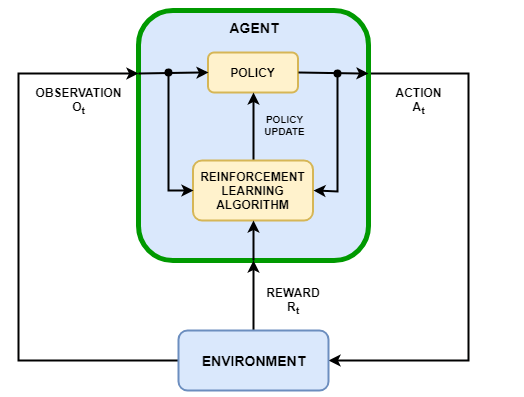
\includegraphics[width = 0.5\linewidth]{figures/MatlabRL.PNG}
    \caption{Rl Environment-Agent Interaction \cite{rl3}}
    \label{fig:my_label}
\end{figure}


\begin{enumerate}

    \item Construct a reset and step function that will be used to construct the environment in which the agent will be in.
    
    \item Define action and Observation information to define how the agent and environment will interact.

    \item The environment was achieved using \textit{rlFunctionenv()} which requires action and observation information as well as the step and reset function.

        \[\textsf{Environment =  rlFunctionenv(ActInf,ObsInf,Stepfunc,Resetfunc)}\]

    \item The agent was constructed using the \textit{rlACAgent()} with the same action and observation options. 
    
    \[\textsf{Agent =  rlACAgent(ActInf,ObsInf)}\]
    
    \item Training options are set Using \textit{rlTainingOptions()} which are used to evaluate the success of an agent, then Agent is trained using \textit{train()}
    
    \[\textsf{TrainingData =  train(Agent,Environment)}\]
    
    \item Agents with the highest cumulative reward are kept.
\end{enumerate} 
 
\clearpage

 \begin{wrapfigure}{r}{0.5\linewidth}
\begin{center}
    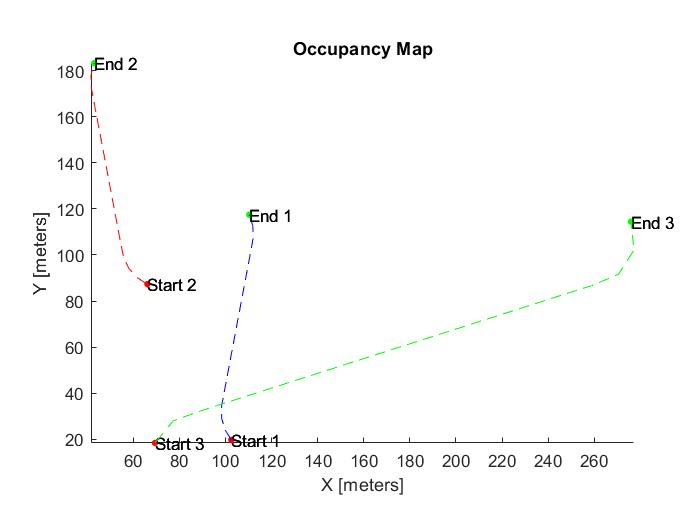
\includegraphics[width=0.45\textwidth]{figures/DroneInitial.jpg}
    \end{center}
    \caption{Environment initial conditions}
    \label{fig:Drone Initial}
\end{wrapfigure}

\subsection{Reset function}
The reset function initiates each episode. It sets the initial positions, velocity, acceleration and endpoints for n drones drone. Figure \ref{fig:Drone Initial} shows the environment 3 drone objects are created at random initial coordinates and 3 corresponding endpoints.

\subsection{Step Function}

\subsubsection{Actions}
From equations, \ref{equ:AtractiveForce}, \ref{equ:sep}, \ref{equ:al} and \ref{equ:coh} in section 2. The control input is the input force to the system so:

\[u_{i} = K_{a_i}\vec{V}_{E_i} + K_{s_i}\vec{V}_{SC_i} + K_{al_i}\vec{V}_{AlC_i} + K_{c_i}\vec{V}_{CD_i} - K_{d_i}\vec{V_i}\]
where:
\[{{\textbf{U}}}(t) = [u_1(t), u_2(t),..., u_N(t)]\]

\noindent
Control signal $U(t)$ is constructed with gains such that:


\begin{align*}
 K_i(t) &= 
    \begin{bmatrix*}[r]
        K_{a_i} & K_{s_i} & K_{al_i} & K_{c_i} & K_{d_i}\\
    \end{bmatrix*}
    V_i(t) = 
    \begin{bmatrix*}
        \vec{V}_{E_i}\\
        \vec{V}_{SC_i}\\
        \vec{V}_{AlC_i}\\
        \vec{V}_{CD_i}\\
        \vec{V}_{d_i}
    \end{bmatrix*}\\
    \centering
\end{align*}
   

where:


\begin{equation}
\begin{split}
    {{\textbf{A}}}(t) &= [K_1(t), K_2(t),..., K_N(t)]\\
    {{\textbf{V}}}(t) &= [V_1(t), V_2(t),..., V_N(t)]\\
    \end{split}
\end{equation}
The agent is able to change gains to vary the behaviour of the system, prioritising certain behaviours. $\textbf{A}(t)$ is the action at each step. The information is constructed using rlNumericSpec() which is used to set the action as a $5\times N$ array of continuous values such that:

\[\textsf{ActionInfo = rlNumericSpec([5 n]);}\]
\[\textsf{ActionInfo.LowerLimit = zeros(5,n)};\]
\[\textsf{ActionInfo.UpperLimit =  ones(5,n)*20;}\]

Reasonable Upper and lower limits were set based on other boid simulations parameters.
\subsubsection{Observations}
As actor-critic networks are a model free approach more than just states spaces can be observed. The observations made are the 5 desired velocities calculated from the boids model as well as position, endpoint and number of flock-mates. This is constructed as follows:

\[O_i = \{V^T_i,\vec{p}_i,\vec{p}_{end},j\in{\cal{F}}_i\}\]

where:

\[V^T_i = \Big[\vec{V}_{E_i}, \vec{V}_{SC_i}, \vec{V}_{AlC_i}, \vec{V}_{CD_i}, \vec{V}_{y_i}\Big]\]

These are all 2 dimensional vectors except for $j\in{\cal{F}}_i$ which is the number of flock-mates for agent i. The x and y coordinates are separated to give:

\[O_i = \Big[V_{E_{ix}}, V_{SC_{ix}}, V_{AlC_{ix}}, V_{CD_{ix}}, V_{d_{ix}}, p_{ix},p_{end_{ix}}, V_{E_{iy}}, V_{SC_{iy}}, V_{AlC_{iy}}, V_{CD_{iy}}, V_{d_{iy}},p_{iy},p_{end_{iy}},j\in{\cal{F}}_i\Big]\]

The full system observation at time step t is constructed as:

\[\textbf{O}(t) = [O_1(t),O_2(t),...O_N(t)]\]

This dimension is defined in MATLAB as:

\[\textsf{ObservationInfo = rlNumericSpec([15 n]})\]

\subsubsection{States: multi-agent  double integrator}
A Multi-agent double integrator model\cite{mul1}  was used to simulate environment dynamics. Let N drones be moving in a 2-Dimensional plane. The linear state-space representation of the double integrator model is then:

\begin{equation}
\begin{aligned}
\dot{\xi}_{i}(t) &= A\xi_i(t) + Bu_i(t)\\
v_{i}(t) &= C\xi_i(t)
\end{aligned}
\end{equation}

\noindent
Where $\xi_i = [x_i,\dot{x}_i,y_i,\dot{y}_i]^T$ and:

\vspace{0.5cm}


\begin{align*}
 A &= 
    \begin{bmatrix*}[r]
        0 & 1 & 0 & 0\\
        0 & 0 & 0 & 0\\
        0 & 0 & 0 & 1\\
        0 & 0 & 0 & 0
    \end{bmatrix*}
    B = 
    \begin{bmatrix*}
        0 & 0\\
        1 & 0\\
        0 & 0\\
        0 & 1
    \end{bmatrix*}\\
    \centering
    C &= 
     \begin{bmatrix*}
        1 & 0 & 0 & 0\\
        0 & 0 & 1 & 0
    \end{bmatrix*}
\end{align*}

\noindent
Here, $v_i$ is the measured output which in this case is the position $(x_i,y_i)$ of the $i^{th}$ drone. This is constructed using the perception radius from equation \ref{equ:per} section \ref{flock}. In this multi agent system agents are aware of relative speed:
\begin{equation}
z_{i}(t) = \sum_{j\in{\cal{F}}_i}(v_i(t) - v_j(t))
\end{equation}

\noindent
For $i = 1...N$, the flock consists of the set ${\cal{F}}_i \subset\{1,2,...N\}/\{i\}$.This then denotes the other drones that the agent $i$ is aware off. The system is:

\begin{equation}
\dot{X}(t)=(I_{N}\otimes A)X(t)+(I_{N}\otimes B)U(t)
\end{equation}

\noindent
where,

\begin{equation}
\begin{split}
    X(t) &= (\xi_1(t), \xi_2(t), ... \xi_N(t))\\
    U(t) &= (u_1(t), u_2(t), ... u_N(t))
    \end{split}
\end{equation}
\noindent
at the network level:
\begin{equation}
Z(t)=({\cal F}\otimes C)X(t)
\end{equation}


\subsection{Reward function}
The reinforcement learning objective from equation \ref{equ:re} section \ref{GOAL}:

\[J(\theta) = \mathbb{E}[\sum_{t=0}^{T-1} r_{t+1}]\]

The reward therefore needs to maximise in the direction of the desired emergent behaviour.\cite{rew1}.

\begin{itemize}
    \item \textbf{Step reward} provided at every step.
    \item \textbf{Episodic reward} is provided at the end of every simulation which occurs at once all agents have arrived or the maximum iterations have been reached. 
\end{itemize}

In this scenario it is the agent should move towards the destination but also flock with other agents as long as this does not sway it too much from its original objective. If the agents are only rewarded for discrete observations such as arriving at a destination or flocking with a member the reward system may be sparse, where the agent receives no signal for long series of actions and observations. To reduce the sparsity of reward, a continuous reward function is designed to push certain behaviours which is incorporated into the step reward function. \cite{shaping}
\clearpage
\subsection{Shaping step reward}
The function $e^{-k_r\sqrt{x^2}}$ is used to construct the reward function.

\begin{figure}[h]
        \centering
   \begin{subfigure}[b]{0.45\textwidth}
         \centering
         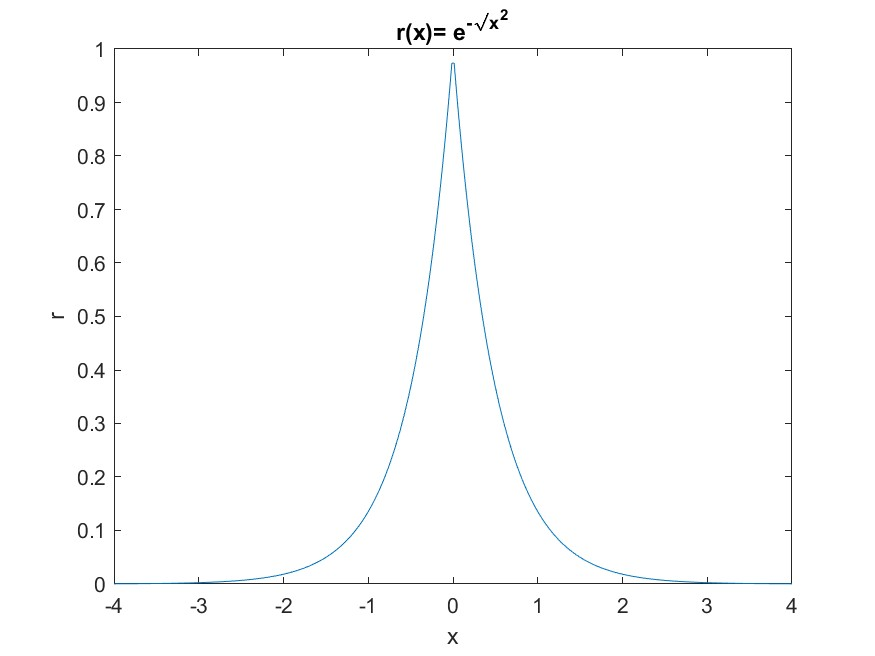
\includegraphics[width=\textwidth]{figures/Exp.jpg}
         \caption{Exponential decay 2D}
         \label{fig:exp1}
     \end{subfigure}
     \hfill
     \begin{subfigure}[b]{0.45\textwidth}
         \centering
         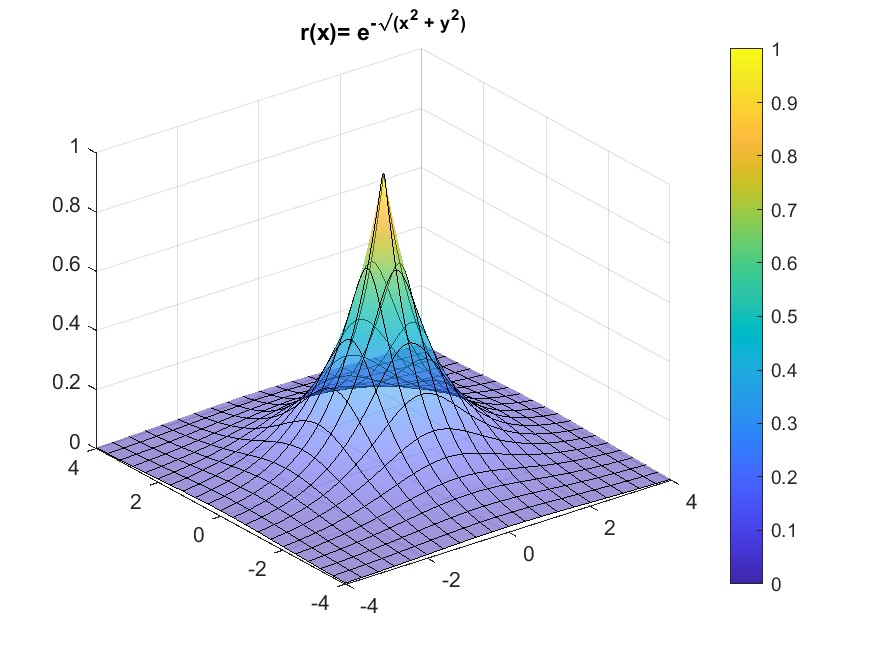
\includegraphics[width=\textwidth]{figures/Exp2.jpg}
         \caption{Exponential decay 3D function }
         \label{fig:exp2}
     \end{subfigure}
     \hfill
\end{figure}

As shown in figures \ref{fig:exp1} and \ref{fig:exp2}, The maximum reward is given at the roots of the function, which in this case are the coordinates of the agent, and tends to 0. This is ideal for a multi-agent system as it allows the control of the size of the horizon of influence of the agents with the constant $k_r$ which is found by applying constraints to the radius of effect and threshold.\hfill\vspace{0.5cm}\\

\noindent
Let the reward function for a point be:

\[r(x,y) = e^{-k_r\rho}\]


Where $\rho = \sqrt{(x-x_{pos})^2 + (y-y_{pos})^2}$. When agent coordinates are equal to the point coordinates:

\[e^0 = 1\]

The maximum area of effect is defined as $\rho_{max}$ and the threshold reward $r_t$ is the reward at $\rho = \rho_{max}$ so:

\[r_t = e^{-k_r\rho_{max}}\]

so:

\[k_r = \frac{ln(r_t)}{\rho_{max}}\]

The reward function of the drones is set to a smaller radius as it is only beneficial to flock when close to another agent. The maximum area of influence is expressed as relative to the size of the map by using the map hypotenuse $h = \sqrt{width^2 + height^2}$. The threshold was set to $r_t = 0.05$ as this meant the signal was only 5\% of the original signal at that point and so had a low effect on change in reward.\vspace{0.5cm}\\
\clearpage
\noindent
\textbf{Flocking reward}\\
\noindent
The flocking reward was chosen  so that the effective area of the drones needed to be smaller than the endpoint effective area so:
\[max(\rho_f) = 0.2h\]
then,
\[k_f = \frac{ln(0.05)}{0.2h}\]

The flocking reward is then the average of all flocking rewards thus,

\begin{equation}
    r_{f_{i}} = \frac{1}{n}\sum_{j=1}^{f} e^{-k_f\sqrt{({x}_i - {x}_j )^2 + ({y}_i - {y}_j)^2}}
    \label{equ:Frew}
\end{equation}


\noindent
\textbf{Endpoint Reward}

\[max(\rho_e) = 0.6h\]
so,
\[k_e = \frac{ln(0.05)}{0.6h}\]

\begin{equation}
    r_{e_i} = e^{-k_e\sqrt{({x}_i - {x}_e )^2 + ({y}_i - {y}_e)^2}}
    \label{equ:Erew}
\end{equation}

\noindent
The sum of these two reward functions is represented in figure \ref{fig:RewardFunc}. See appendix A1 for more details.

\begin{figure}[h]
  \begin{center}
    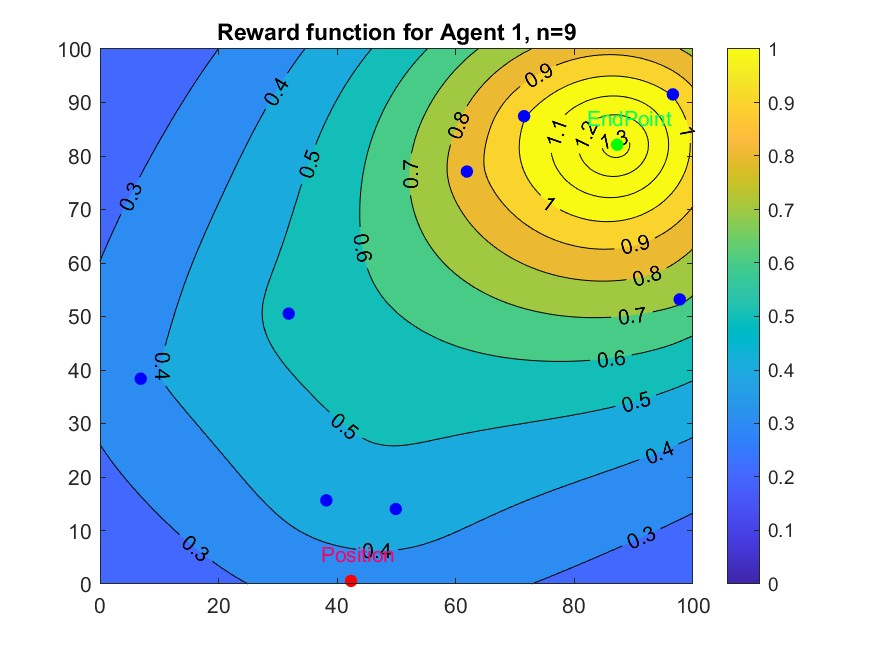
\includegraphics[width=0.60\textwidth]{figures/Reward.jpg}
    \end{center}
    \caption{Reward function with 9 agents}
    \label{fig:RewardFunc}
\end{figure}
\clearpage
\noindent
\textbf{Penalty}\newline
From equation \ref{equ:rew} cumulative return for time step k is:

\[r_t^\gamma = \sum_{k =  t}^T\gamma^{n-t}r(s_k,a_k)\]

If $0 < \gamma < 1$ and the $r > 0$ then it can be seen that $r^\gamma$ tends to 0. This implies the maximisation problem is impossible. To solve this, a penalty is added to the step function to push the agent to arrive within a set number of steps defined as $T_{max}$.  The exponential function $ae^{-k_{p}x}$ is used as constants a and $k_p$ can be changed to form the appropriate signal. For the agent to arrive within $T_{max}$ steps the following definition is formulated:
\begin{center}
    \(r_t = 0\) for \(t = T_{max}\)
\end{center}

Total step reward $r_t$ is the sum of equations \ref{equ:Frew} and \ref{equ:Erew} minus the penalty.

\[r_{t_i} = r_{f_i} + r_{e_i} - r_{p_i} = 0\]
where:
\[r_{p_i} = ae^{k_{p}T_{max}}\]
and maximum possible values for $r_{f_i}$ and $r_{e_i}$ is 1. Through substitution this yields:

\[ae^{k_{p} T_{max}} = 2\]

Applying initial conditions a is found:
\begin{center}
    \(ae^0 = a\) where a is set so that \(a << 2,\)
\end{center}


Applying terminal conditions:
\begin{equation}
    k_{p} = \frac{ln(\frac{2}{a})}{T_{max}}
    \label{equ:kp}
\end{equation}
Note that $r_{f_i}$ the sum of $r_{e_i}$ is only equal to 2 when all reward functions are at the same point which is unlikely. It is better to overestimate, however, as this prevents exponential growth of the reward.
\begin{figure}[h]
    \centering
    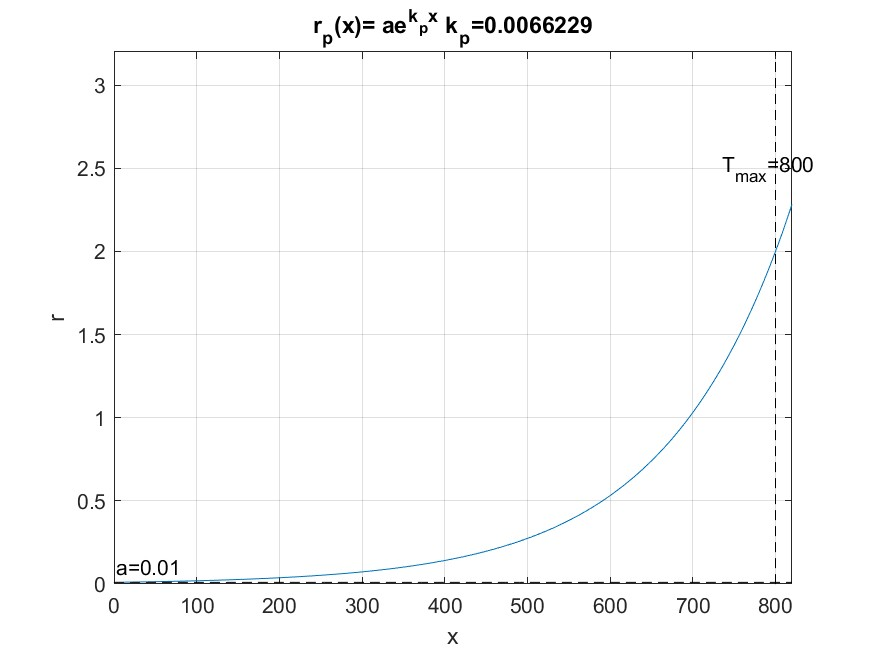
\includegraphics[width=0.4\textwidth]{figures/Exp3.jpg}
    \caption{Penalty function}
    \label{fig:exp3}
\end{figure}\\
Figure \ref{fig:exp3} shows the penalty function used. The reward for each agent step is then:
\[r_{t_i} = r_{f_i} + r_{e_i} - r_{p_i}\]

The total reward for each simulations time step $n$ is then the average reward of the N agents:
\[r_{step_n} = \frac{1}{N}\sum_{i=1}^{N}r_{t_i}\]


\subsection{Episodic reward}

The episodic reward takes into account the overall success of the simulation, providing this reward once a maximum number of steps is achieved or all agents have arrived at their destinations. This is represented as:

\[R_{total} = r_{episodic} + \sum^T_{n=1}{r_{step_n}}\]

The episodic reward is based of the terminal state of the system.
It takes number of individuals that have arrived at their destinations such that if agent i has arrived within a set arrival distance:
\[r_{a_i} = 1\]
And if agent i hasn't arrived:
\[r_{a_i} = 0\]

Then total episodic reward is 
\[r_{episodic} = \frac{1}{N}\sum_{i=1}^{N}r_{a_i}\]

The overall maximisation problem becomes:

\[MaxJ(\theta) = max(R_{total})\]










\subsection{Training Options}

Knowing the maximum cumulative reward that is achievable is important as it sets limits as to what outcome to expect. The reinforcement learning toolbox provides the \(rlTrainingOptions()\) allows us to define the criteria for a well-trained agent as well as limit the number of steps per episode.\\


\begin{center}
    \textsf{trainOpts = rlTrainingOptions('MaxStepsPerEpisode',800,...\\'SaveAgentCriteria','EpisodeReward','SaveAgentValue',800);}\\
\end{center}


\noindent
This limits the maximum number of steps per episode as well as specifies that an agent with a cumulative reward of \(J(\theta) = 1050\)  is a successful agent.